\documentclass[oneside, final, 10pt]{extarticle}
\usepackage[utf8]{inputenc}
\usepackage[russian]{babel}
\usepackage{vmargin}
\usepackage{listings}
\usepackage{graphicx}
%\usepackage{ucs}
\setpapersize{A4}
\setmarginsrb{2cm}{2cm}{2cm}{2cm}{0pt}{0mm}{0pt}{13mm}
\usepackage{indentfirst}		%красная строка
%\usepackage{color}
\sloppy

\begin{document}
\begin{titlepage}
	\begin{centering}
		\textsc{Министерство образования и науки Российской Федерации}\\
		\textsc{Новосибирский государственный технический университет}\\
		\textsc{Кафедра теоритической и прикладной информатики}\\
	\end{centering}
	%\centerline{\hfill\hrulefill\hrulefill\hfill}
	\vfill
	\vfill
	\vfill
	\Large
	\centerline{Лабораторная работа №1}
	\centerline{по дисциплине "<Компьютерная графика">}
	\centerline{\bfВведение в программирование}
	\centerline{\bfс использованием OpenGL}
	\normalsize
	\vfill
	\vfill
	\vfill
	\begin{flushleft}
		\begin{minipage}{0.3\textwidth}
			\begin{tabular}{l l}
				Факультет: & ПМИ\\
				Группа: & ПМИ-41\\
				Студент: & Кислицын И. О.\\
				Преподаватель: & Задорожный А. Г.\\
			\end{tabular}
		\end{minipage}
	\end{flushleft}
	\vfill
	\vfill
	\begin{centering}
		Новосибирск\\
		2017\\
	\end{centering}
\end{titlepage}
\setcounter{page}{2}
\lstset{
	breaklines=\true,
	%frame=single,
	basicstyle=\footnotesize\ttfamily,
	tabsize=2,
	showspaces=\false,
	showstringspaces=\false,
	breaklines=\true,
	breakatwhitespace=\true,
	%escapeinside={"}{"},
	%inputencoding=utf8x,
	extendedchars=\true,
	keepspaces=\true
}
\section{Цель работы}

Ознакомиться с основами использования библиотеки \verb~OpenGL~ и работе с примитивами.

\section{Задача}

Написать программу, отображающую множество примитивов, вершины которых задаются кликами мыши.

\section{Описание разработанной программы}

\begin{figure}[t]
	\centering
	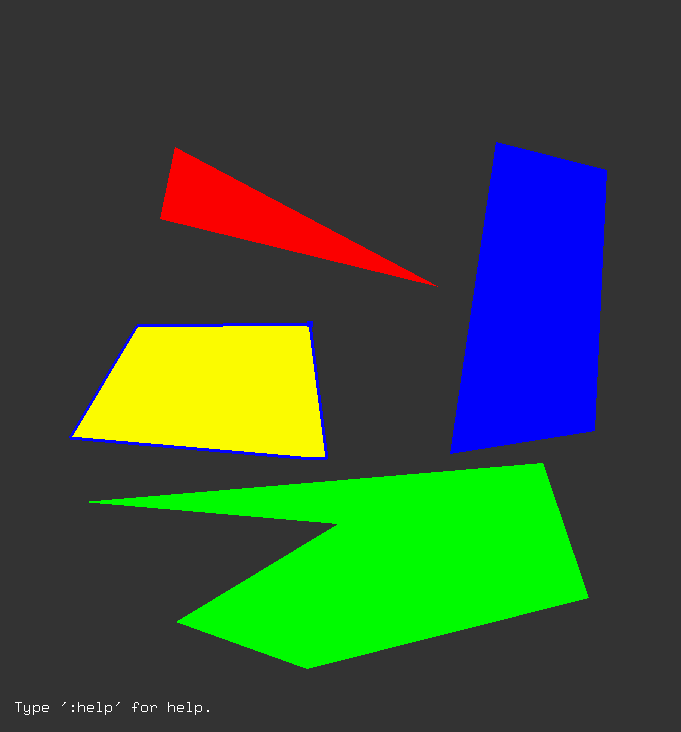
\includegraphics[width=0.9\textwidth]{screen/iface}
	\caption{Интерфейс программы}
	\label{iface}
\end{figure}

Программа позволяет рисовать многоугольники с помощью примитива \verb~GL_POLYGON~. Текущий (редактируемый) многоугольник выделяется с помощью контура, последняя поставленная точка выделяется размером.

\subsection{Запуск программы}

Для запуска программы необходим \verb~python 2.7~. Запуск производится командой \verb~python lab1.py~.

\subsection{Управление}

Все команды с клавиатуры вводятся в латинской раскладке. Заглавная буква означает, что клавишу нужно нажимать с зажатой клавишей \verb~Shift~.

\begin{itemize}
	\item \verb~Left Mouse Button~~-- добавить точку к многоугольнику.
	\item \verb~Right Mouse Button~~-- удалить выделенную точку из многоугольника.
	\item \verb~Middle Mouse Button~~-- завершить многоугольник.
	\item \verb~w, a, s, d~~-- переместить выделенную точку многоугольника.
	\item \verb~W, A, S, D~~-- переместить текущий многоугольник.
	\item \verb~r, g, b~~-- увеличить значение соответствующего канала цвета текущего многоугольника.
	\item \verb~R, G, B~~-- уменьшить значение соответствующего канала цвета текущего многоугольника.
	\item \verb~',', '.'~~-- выделить следующую точку.
	\item \verb~<, >~~-- выделить следующий многоугольник.
	\item \verb~:~~-- перейти в режим командной строки.
\end{itemize}

\subsection{Режим командной строки}

В режиме командной строки доступны следующие команды:

\begin{itemize}
	\item \verb~:help~~-- вывести на экран информацию об управляющих клавишах.
	\item \verb~:get param~~-- вывести значение параметра \verb~param~. Список доступных параметров см. в разделе \ref{param}.
	\item \verb~:set info~~-- вывести список доступных параметров.
\item \verb~:set param value~~-- изменить значение параметра \verb~param~ на \verb~value~. Список доступных параметров и их возможных значений см. в разделе \ref{param}.
	\item \verb~:clear~~-- отчистить экран от текста.
\end{itemize}

\subsection{Параметры} \label{param}

\begin{itemize}
	\item \verb~title~~-- заголовок окна (доступен для изменения только с помощью файла конфигурации).
	\item \verb~bg~~-- цвет фона в формате \verb~#rrggbb~ (по умолчанию \verb~#333333~).
	\item \verb~text_color~~-- цвет текста в формате \verb~#rrggbb~ (по умолчанию \verb~#ffffff~).
	\item \verb~shape_color~~-- цвет заливки фигуры в формате \verb~#rrggbb~ (по умолчанию \verb~#000000~).
	\item \verb~motd~~-- текст, который выводится на экран при начале работы с приложением (по умолчанию \verb~"Type ':help' for help."~).
	\item \verb~point_size~~-- размер точки, обозначающей текущую вершину (по умолчанию \verb~6~).
	\item \verb~line_width~~-- толщина контура текущего многоугольника (по умолчанию \verb~3~).
	\item \verb~color_delta~~-- значение, на которое изменится цвет многоугольника при использовании клавиш \verb~r, g, b (R, G, B)~ (по умолчанию \verb~5~).
	\item \verb~pos_delta~~-- значение, на которое переместится точка/многоугольник при использовании клавиш \verb~w, a, s, d~/\verb~W, A, S, D~ (по умолчанию \verb~9~).
\end{itemize}

\subsection{Файл конфигурации}

Для исполнения набора команд при каждом запуске системы используется файл \verb~./.lab1rc~. Команды в файл записываются по одной на строку без символа \verb~:~. Например:

\lstset{caption=.lab1rc}
\lstinputlisting{.lab1rc}

Результат загрузки программы с данным \verb~.lab1rc~ изображён на скриншоте \ref{rcd}.

\begin{figure}[t]
	\centering
	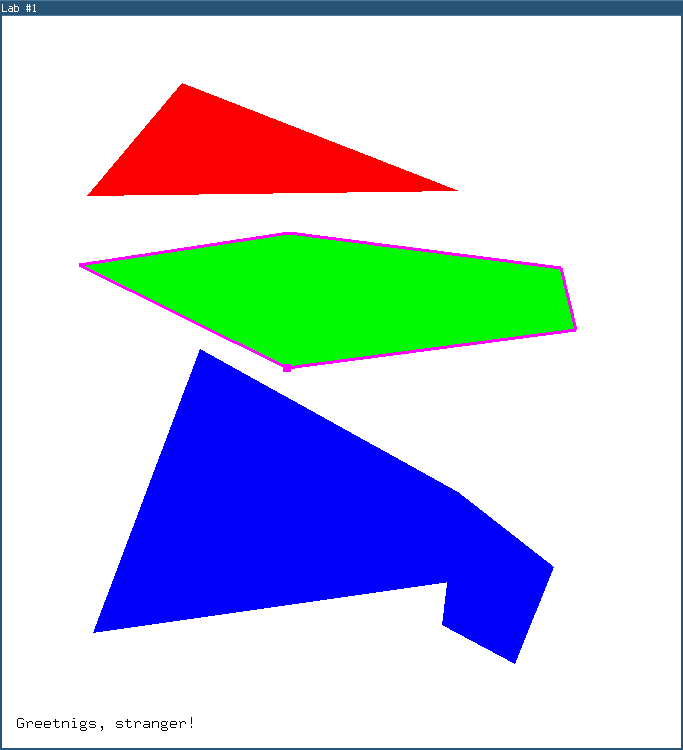
\includegraphics[width=0.9\textwidth]{screen/rcd}
	\caption{Интерфейс программы (изменённый .lab1rc)}
	\label{rcd}
\end{figure}

\section{Текст программы}

\lstset{caption=lab1.py}
\lstinputlisting[language=python]{main.py}

\end{document}
